\chapter{Conceptual framework} \label{Chp:Concepts}

This chapter describes the conceptual framework of the method used by \dfastmi.
It all starts with the design of a river intervention, i.e.~a local river adjustment, to address some issue e.g. an adjustment to increase the flow capacity.
In order to evaluate the intervention, it's important to also look at the morphological changes caused by the changing flow patterns.
\dfastmi implements algorithms to provide an estimate of the long-term morphological effect inside the main channel, as well as the degree to which this adjustment may occur in the first year.
The next couple of sections provide context and theory to underpin the implemented algorithms.
\Autoref{Sec:Limitations} provides an overview of the assumptions and limitations of this tool.


\section{Characteristics of bed level changes due to river interventions}

A river intervention, i.e.~a local river adjustment (typically a flow capacity enlarging adjustment) outside the main channel, may result in changes in the flow pattern within the main channel.
The bed levels within the main channel will react to such changes depending on the magnitude, duration and length scale of these flow pattern changes in the main channel.

Hence, the core focus of the rule-of-thumb is to determine and characterize the changes in the flow pattern within the main channel.
Here, we define the main channel as the part of the river between the groyne heads.

At the upstream end of the floodplain adjustment part of the main channel discharge will leave the main channel, which will flow through the enlarged floodplain, secondary channel or bank area, and return to the main channel at the downstream end of the project area.
The resulting changes in the main channel flow pattern cause sedimentation in the main channel at the upstream "offtake" of the new outflow and erosion at the downstream "confluence" when the flow enters the main channel again.
See \autoref{Fig:response}.
Because the river discharge varies, the pattern will also vary during the year.
As a result a part of the main channel bed level adjustment is stationary and a part of the adjustment is transitional and it will migrate downstream.
A reduction in the water depth may thus not only be observed locally where the flow diverges into the flood plain, but also downstream thereof.

\begin{figure}
\center
\resizebox{13cm}{!}{
   \input{figures/response.pdf_tex}
}
\caption{Equilibrium and initial response under steady discharge}
\label{Fig:response}
\end{figure}

The bed level change due to river enlargement can largely be characterized as follows

\begin{itemize}
\item The magnitude of the bed level change varies over the seasons; the maximum change is observed at the end of the flood season and the adjustment reaches a minimum at the end of the low flow period.

\item Local evaluation of the bed level changes is insufficient because of partial downstream migration of the bed level changes.

\item The maximum impact is observed on that side of the river which is closest to the adjustment.
\end{itemize}

Because part of the bed level changes migrate downstream, the morphological impact on projects located downstream may be increased.
After all, the maximum bed level change of one single river enlarging intervention is reached at the end of the flood period and it's the result of that flood period.
However, when a series of interventions along the river are combined (for instance, lowering of the groynes along a reach) the downstream bed level changes may be increased by accumulation of downstream migrating bed waves, such that the accumulated bed level change may be significantly larger.
In other words, river interventions extending over longer reaches may result in a larger morphodynamic response than comparable but more isolated interventions.

The aforementioned observations result in the following premises.
The rule-of-thumb described in the following sections

\begin{itemize}
\item will only be valid for the estimation of the impact of local interventions with a length of at most one flood plain,

\item should take into account seasonal variations, and

\item needs to be estimate the spatial pattern of the bed level change.
\end{itemize}


\section{Characterization of the changes in the main channel flow pattern}

When an intervention in the floodplains does not include something like a permanently active secondary channel, the flow pattern in the main channel will only be affected during flood conditions.
If on the other hand, such a secondary channel (or other intervention active under medium to low flow conditions such as groyne adjustments) is included in the design then the flow pattern will also be influenced during transitional or even low flow conditions.
It's therefore critical to determine the effect of the intervention on the main channel flow pattern at different discharge levels.

Secondary channels may have a major impact on the morphodynamics of the main channel.
The magnitude of the discharge through the secondary channel varies as function of the river discharge.
Because the hydraulic conditions of the secondary channel can change over time (e.g.~due to vegetation, siltation, or erosion) the discharge through a secondary channel is typically controlled by some hydraulic structure.
The typical characteristics of a weir (Dutch: overlaat, drempel) and orifice (Dutch: onderlaat, duiker) are shown in \autoref{Fig1}.

\begin{figure}[b]
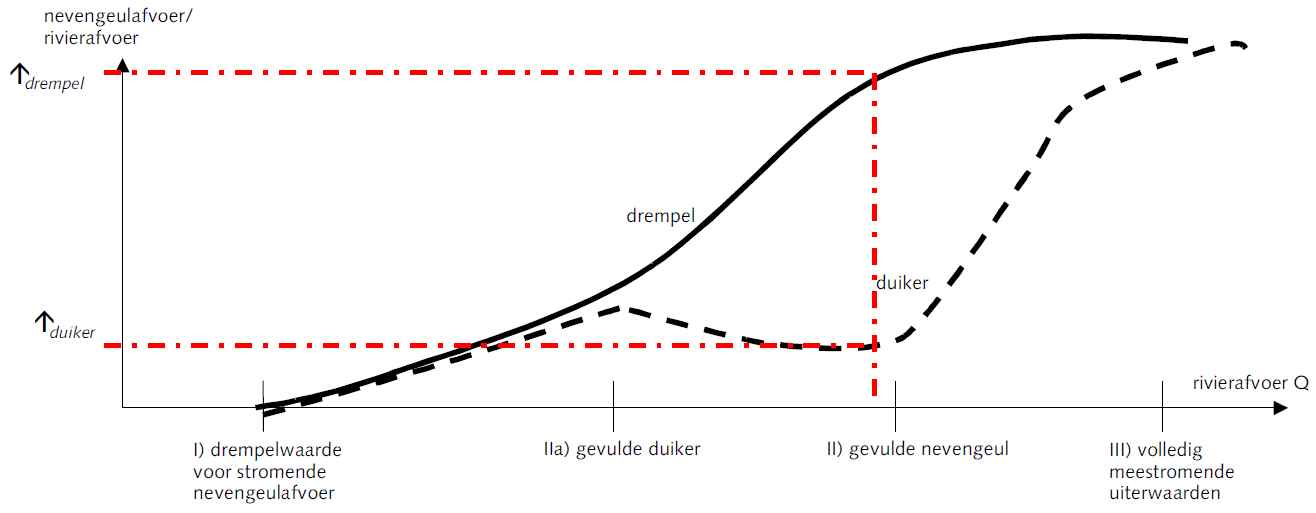
\includegraphics[width=\columnwidth]{figures/Fig1.png}
\caption{Schematic of the controlled discharge through a secondary channel.}
\label{Fig1}
\end{figure}

The discharge through a secondary channel is characterized by a number of special conditions as illustrated by \autoref{Fig1}:

\begin{enumerate}
\item the beginning of flow through the secondary channel
\item the bankfull secondary channel
\item the fully developed flow in the secondary channel and surrounding floodplain.
\end{enumerate}

When the discharge through the secondary channel is controlled by an orifice, the fully flooded condition may add an additional characteristic discharge.
In order to characterize the flow patterns during flood it's necessary to distinguish the condition in which the flood plains just start to carry flows, and the condition of fully developed flow in the flood plains.
\dfastmi version 2 and before (in WAQMORF) used an algorithm to determine which three flow conditions would best represent the effect of the intervention under various conditions.
However, as these conditions varied depending on the thresholds specified by the user, the tool could give different results depending on the user.
In \dfastmi version 3, a new method has been implemented that removes most input parameters; only the threshold discharge at which the intervention starts affecting the flow velocities in the main channel, besides the general location characteristics of the branch and reach in which the intervention is located.


\section{Equilibrium bed level change: the discharge dominated case}

\dfastmi is based on a highly simplified model of river morphodynamics.
The derivation of the algorithm starts by assuming a quasi-stationary flow pattern and an outflow of discharge and sediment from the main channel while the local water level is independent of the hydraulic and morphological changes in the main channel (a \emph{rigid-lid} approximation).
Note that the outflow of sediment is assumed to be a consequence of the outflow of discharge only; the conceptual framework does not allow for selective removal of only sediments.
%
\begin{align}
&\text{water} & \pdiff{q_\text{mc}}{s} = -q_\text{out} \label{Eq:MassConcWater} \\
&\text{sediment} & \pdiff{z_b}{t} + \pdiff{s_\text{mc}}{s} = -s_\text{out} \label{Eq:MassConcWater}
\end{align}
%
in which
%
\begin{symbollist}
\item[$q_\text{mc}$] main channel discharge per unit width \unitbrackets{m\textsuperscript{2} s\textsuperscript{-1}}
\item[$q_\text{out}$] discharge per channel unit width \emph{to} the flood plain per unit river length \unitbrackets{m\textsuperscript{2} s\textsuperscript{-1} m\textsuperscript{-1}}
\item[$s$] stream-wise coordinate \unitbrackets{m}
\item[$z_b$] bed level change due to intervention \unitbrackets{m}
\item[$s_\text{mc}$] main channel sediment transport per unit width \unitbrackets{m\textsuperscript{2} s\textsuperscript{-1}}
\item[$s_\text{out}$] sediment transport per channel unit width \emph{to} the flood plan per unit river length \unitbrackets{m\textsuperscript{2} s\textsuperscript{-1} m\textsuperscript{-1}}
\end{symbollist}
%
The response of the main channel is represented here by a bed level change $\Delta z_b$ \unitbrackets{m} (raise or lowering) which is small relative to the local water depth.
The sediment transport capacity per unit width of the main channel, $s_\text{mc}$, is approximated by $s_\text{mc} = m \left ( q_\text{mc} / h \right )^b$ with $h$ the water depth \unitbrackets{m} in the main channel, $m$ a calibration factor \unitbrackets{m\textsuperscript{2-b} s\textsuperscript{b-1}} and a dimensionless sediment transport exponent $b$, which is 5 for \citet{Engelundh67}.
Based on these equations, one can derive that the bed level development during such a period of constant discharge is given by the following relaxation
%
\begin{equation}
\Delta z_b = \Delta z_b (0) + [\Delta z_{b,\text{eq}} - \Delta z_b(0)](1 - e^{-t/T_m})
\label{Eq:zbRelax}
\end{equation}
%
where the morphological time scale $T_m$ is given by
%
\begin{equation}
T_m = \frac{L}{c} \approx \frac{h L}{b s_\text{mc}}
\label{Eq:MorTimeScale}
\end{equation}
%
where $c$ is the bed celerity \unitbrackets{\SI{}{\metre\per\second}} ($\approx b s_\text{mc} / h$), and the equilibrium bed level change $\Delta z_{b,\text{eq}}$ (for one steady flow forcing) equals the product of the water depth and the relative change in the main channel velocity $u$ \unitbrackets{m/s}
%
\begin{equation}
\Delta z_{b,\text{eq}} \approx -h \left ( \frac{\Delta u}{u} \right )
\label{Eq:zbEqui}
\end{equation}
%
The easiest way to understand this equation is to realize that it states that the velocity change caused by the intervention will be compensated by a bed level change such that the velocity, and hence the sediment transport capacity, returns to the original value.
Note that we have assumed that the effect on the water level is negligible, hence the water depth change $\Delta h$ equals the bed level change $\Delta z_{b,\text{eq}}$.
%
\begin{equation}
\Delta h u + h \Delta u \approx 0.
\label{Eq:zbEqui2}
\end{equation}
%
In reality the discharge isn't constant throughout the year.
Instead, the year is assumed to be represented by a hydrograph series of constant discharges.
The bed level development during a single period of the hydrograph is given by \autoref{Eq:zbRelax}, such that at the end of period $i$ (lasting $T_i$ days) the morphological effect of the intervention is given by
%
\begin{equation}
\Delta z_{b,i+1}(0) = \Delta z_{b,i} (0) \sigma_i + \Delta z_{b,i,\text{eq}} (1-\sigma_i) \text{ with } \sigma_i = e^{-T_i/T_{m,i}}
\label{Eq:zbOverTime}
\end{equation}
%
Let $N$ be the number of periods of constant flow occurring in the order from $i=1$ to $i=N$ in the hydrograph; each period $i$ may have a different duration $T_i$.
Note that the same discharge may occur multiple times during the hydrograph and there may be multiple peaks and lows in the hydrograph.
The initial bed level change $\Delta z_{b,i}(0)$ of a period $i$ equals the final bed level change $\Delta z_{b,i-1}(T_{i-1})$ of the preceding period $i-1$.
This gives a set of $N$ equations with $N$ unknowns $\Delta z_{b,i}(0)$ for the dynamic long-term equilibrium if we assume that the final bed level of the last period $\Delta z_{b,N}(T_N)$ or $\Delta z_{b,N+1}(0)$ equals the initial bed level of the first period $\Delta z_{b,1}(0)$.
%
\begin{equation}
\Delta z_{b,i+1}(0) = \Delta z_{b,i}(0) \sigma_i + \Delta z_{b,i,\text{eq}} (1-\sigma_i) \text{ for $i$ equals 1 to $N$}
\label{Eq:zbiNPeriods}
\end{equation}
%
This set of equations can be solved for $\Delta z_{b,i}(0)$ giving
%
\begin{equation}
\Delta z_{b,i}(0) = \frac{1}{\xi} \sum_{j=0}^{N-1} \Delta z_{b,i+j,\text{eq}} (1-\sigma_{i+j}) \prod_{k=j+1}^{N-1} \sigma_{i+k}
\end{equation}
%
where $\xi = 1 - \prod_{i=1}^N \sigma_i$ and all indices $m>N$ are equivalent to $m-N$ for reasons of periodicity.
If the impact of the intervention increases as the discharge increases, the maximum bed level change is likely reached at the end of the period with the highest discharge.
However, this isn't true for all hydrographs and for all interventions.
Similarly, the minimum bed level change is frequently reached at the end of the period with the lowest discharge, but this may also depend on the details of the hydrograph used (which may for instance include multiple low flow periods of different duration).
For this reason, the minimum and maximum values are determined independently for every individual grid cell as the minimum and maximum over all $N$ fields of $\Delta z_{b,i}(0)$.
The year-averaged bed level change $\bar{\Delta z_b}$ at long-term dynamic equilibrium can be computed as
%
\begin{equation}
\bar{\Delta z_b} = \frac{\sum{\Delta z_{b,i,\text{eq}} T_i}}{\sum{T_i}} + \frac{\sum{(\Delta z_{b,i,\text{eq}} - \Delta z_{b,i}(0)) T_{m,i} (\sigma_i-1)}}{\sum{T_i}}
\label{Eq:zbMean}
\end{equation}
%
More details are given in \citet{JagersGiri2022}.


\section{Equilibrium bed level change: extending to tides}\label{Sec:Tides}

The concept of the ``hydrograph'' consisting of $N$ periods of constant forcing.
The forcing could besides the discharge that was discussed above, also include the downstream water level (storm surge and tidal conditions).
Although the current \dfastmi version includes code preparations for such extensions; the application domain is, for the time being, limited to the river reaches where such effect can be ignored.


\section{Estimate for dredging volumes}\label{Sec:DredgeVol}

An order-of-magnitude estimate of the dredging (or dumping) volume $V_\text{dredge,1yr}$ that will required to keep the bed levels at the initial\footnote{If the bed levels in the main channel differ between the reference simulation and the simulation with the intervention, the level meant here is the bed level as included in the simulation \emph{with} the intervention.} level can be obtained by accumulating the year-averaged equilibrium bed level change $\bar{\Delta z_b}$ (see \autoref{Eq:zbMean}) over the impacted length $L_s$.
In a 1D setting with $x$ indicating the alongstream coordinate \unitbrackets{m}, we can write that down as
%
\begin{equation}
V_\text{dredge,1yr} = \int_{x_0}^{x_0 + L_s} \bar{\Delta z_b}(x) dx
\end{equation}
%
where $x_0$ marks the upstream border of the impacted reach.
The impacted length $L_s$ is defined as the distance over which a bed level disturbance can travel during the part of the year that the flow conditions are different due to the intervention being evaluated, i.e.
%
\begin{equation}
L_s = \sum_{i \text{ where $Q_i > Q_\text{thr}$}} c_i T'_i
\end{equation}
%
where $i$ loops over the conditions for which the discharge $Q_i$ is larger than minimum flow-carrying discharge $Q_\text{thr}$.
The rivers configuration file specifies for each flow condition $i$ the period $T_i$ and celerity $c_i$.
These values are thus given and should not be changed.
The effective morphological period $T'_i$ is equal to the period $T_i$ except for the first flow condition for which the discharge $Q_i$ is larger than minimum flow-carrying discharge $Q_\text{thr}$.
For that condition the period is adjusted based on the discharge exceedance curve (given by \keyw{QFit} in the \nameref{sec:rivers-config}).
The minimum flow-carrying discharge $Q_\text{thr}$ is thus the only parameter given by the user that affects the impacted length.
The sediment transport during the remainder of the year may adjust the shape and location of the deposit, but the total volume remains the same.

It is foreseen that this estimate may be computed automatically in a future release of \dfmi, but this is currently left as a manual step for the user.
In case the intervention triggers multiple separate sedimentation (or erosion) areas, the volumes should be accumulated for each area individually, i.e. not only the most upstream area should be considered, and subsequently the total volume can be accumulated over all areas.
